\documentclass[10pt,a4paper]{article}
\usepackage[UTF8,fontset = windows]{ctex}
\setCJKmainfont[BoldFont=黑体,ItalicFont=楷体]{华文中宋}
\usepackage{amssymb,amsmath,amsfonts,amsthm,mathrsfs,dsfont,graphicx}
\usepackage{ifthen,indentfirst,enumerate,color,titletoc}
\usepackage{tikz}
\usepackage{multicol}
\usepackage{makecell}
\usepackage{longtable}
\usepackage{ifthen}
\usetikzlibrary{arrows,calc,intersections,patterns,decorations.pathreplacing,3d,angles,quotes}
\usepackage[bf,small,indentafter,pagestyles]{titlesec}
\usepackage[top=1in, bottom=1in,left=0.8in,right=0.8in]{geometry}
\renewcommand{\baselinestretch}{2}
\newtheorem{defi}{定义~}
\newtheorem{eg}{例~}
\newtheorem{ex}{~}
\newtheorem{rem}{注~}
\newtheorem{thm}{定理~}
\newtheorem{coro}{推论~}
\newtheorem{axiom}{公理~}
\newtheorem{prop}{性质~}
\newcommand{\blank}[1]{\underline{\hbox to #1pt{}}}
\newcommand{\bracket}[1]{(\hbox to #1pt{})}
\newcommand{\onech}[4]{\par\begin{tabular}{p{.9\textwidth}}
A.~#1\\
B.~#2\\
C.~#3\\
D.~#4
\end{tabular}}
\newcommand{\twoch}[4]{\par\begin{tabular}{p{.46\textwidth}p{.46\textwidth}}
A.~#1& B.~#2\\
C.~#3& D.~#4
\end{tabular}}
\newcommand{\vartwoch}[4]{\par\begin{tabular}{p{.46\textwidth}p{.46\textwidth}}
(1)~#1& (2)~#2\\
(3)~#3& (4)~#4
\end{tabular}}
\newcommand{\fourch}[4]{\par\begin{tabular}{p{.23\textwidth}p{.23\textwidth}p{.23\textwidth}p{.23\textwidth}}
A.~#1 &B.~#2& C.~#3& D.~#4
\end{tabular}}
\newcommand{\varfourch}[4]{\par\begin{tabular}{p{.23\textwidth}p{.23\textwidth}p{.23\textwidth}p{.23\textwidth}}
(1)~#1 &(2)~#2& (3)~#3& (4)~#4
\end{tabular}}
\begin{document}

\begin{enumerate}[1.]

\item 如图, 观察长方体$ABCD-A_1B_1C_1D_1$中的点、线、面, 用适当的符号或字母填空:
\begin{center}
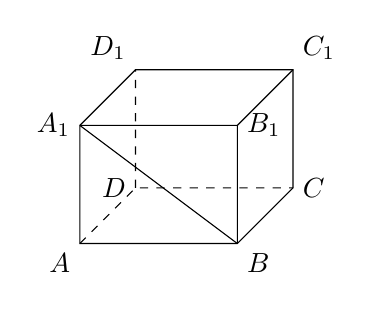
\begin{tikzpicture}[>=latex]
\draw (0,0) node [below left] {$A$} coordinate (A) --++ (2,0) node [below right] {$B$} coordinate (B) --++ (45:{2/2}) node [right] {$C$} coordinate (C)
--++ (0,1.5) node [above right] {$C_1$} coordinate (C1)
--++ (-2,0) node [above left] {$D_1$} coordinate (D1) --++ (225:{2/2}) node [left] {$A_1$} coordinate (A1) -- cycle;
\draw (A) ++ (2,1.5) node [right] {$B_1$} coordinate (B1) -- (B) (B1) --++ (45:{2/2}) (B1) --++ (-2,0);
\draw [dashed] (A) --++ (45:{2/2}) node [left] {$D$} coordinate (D) --++ (2,0) (D) --++ (0,1.5);
\draw (A1) -- (B);
\end{tikzpicture}
\end{center}
(1) 点$B$\blank{20}直线$BC$;\\
(2) 点$A$\blank{20}直线$BC$;\\
(3) 点$D$\blank{20}平面$ABCD$;\\
(4) 点$A_1$\blank{20}平面$ABCD$;\\
(5) 直线$A_1B\cap$直线$BC=$\blank{20};\\
(6) 直线$A_1B\cap$平面$A_1B_1C_1D_1=$\blank{20};\\
(7) 直线$B_1C_1$\blank{20}平面$BB_1C_1C$.
\item 用集合符号表述下列语句, 并将语句所描述的图形画在图中:\\
\begin{center}
\begin{tikzpicture}[>=latex]
\draw (0,0) -- (3,0) --++ (1,1.5) ++ (-0.5,0) node [below] {$\beta$} ++ (0.5,0) --++ (-3,0) -- (0,0);
\draw (0,0) --++ (-1.5,2) --++ (1,1.5) ++ (0.1,-0.2) node [below] {$\alpha$} ++ (-0.1,0.2) --++ (1.5,-2);
\end{tikzpicture}
\end{center}
(1) 点$A$在平面$\alpha$上:\blank{50};\\
(2) 平面$\alpha$经过直线$AC$:\blank{50};\\
(3) 点$B$不在平面$\beta$上:\blank{50};\\
(4) 直线$BC$平行于平面$\beta$:\blank{50}.
\item 下列图形一定是平面图形吗? 请说明理由.\\
(1) 三角形;\\
(2) 梯形;\\
(3) 四边形;\\
(4) 菱形.
\item 判断下列命题的真假:\\
(1) 若空间四点共面, 则其中必有三点共线;\\
(2) 若空间四点中有三点共线, 则此四点必共面;\\
(3) 若空间四点中任何三点不共线, 则此四点不共面;\\
(4) 若空间四点不共面, 则其中任意三点不共线.
\item 证明公理2后的推论2.
\item 平面$\alpha$与平面$\beta$相交于直线$l$, 点$A$、$B$在平面$\alpha$上, 点$C$在平面$\beta$上但不在直线$l$上, 直线$AB$与直线$l$相交于点$R$. 设$A$、$B$、$C$三点确定的平面为$\gamma$, 则$\beta$与$\gamma$的交线是\bracket{20}.
\begin{center}
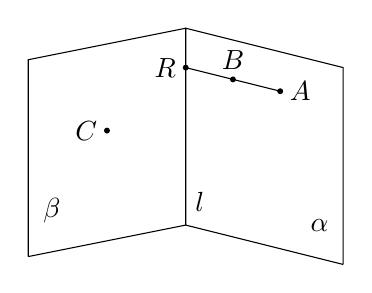
\begin{tikzpicture}[>=latex]
\draw (0,0) -- (2,-0.5) ++ (-0.3,0.3) node [above] {$\alpha$} ++ (0.3,-0.3) --++ (0,2.5) --++ (-2,0.5) -- (0,0) ++ (0,0.3) node [right] {$l$};
\draw (0,0) -- (-2,-0.4) ++ (0.3,0.3) node [above] {$\beta$} ++ (-0.3,-0.3) --++ (0,2.5) --++ (2,0.4);
\filldraw (0,2) circle (0.03) node [left] {$R$} coordinate (R);
\filldraw (1.2,1.7) circle (0.03) node [right] {$A$} coordinate (A);
\filldraw ($(A)!0.5!(R)$) circle (0.03) node [above] {$B$} coordinate (B);
\draw (A) -- (R);
\filldraw (-1,1.2) circle (0.03) node [left] {$C$} coordinate (C);
\end{tikzpicture}
\end{center}
\fourch{直线$AC$}{直线$BC$}{直线$CR$}{以上均不正确}
\item 如图, 已知直线$l$与平面$\alpha$相交于点$O$, $A$、$B \in l$, $C$、$D\in \alpha$, 且$AC\parallel BD$. 求证: $O$、$C$、$D$三点共线.
\begin{center}
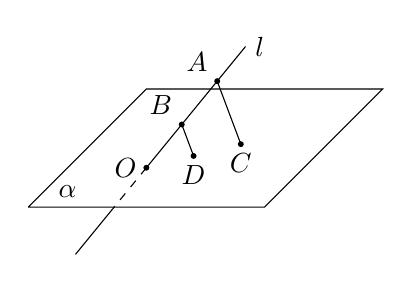
\begin{tikzpicture}[>=latex]
\draw [name path = plane] (0,0) -- (3,0) -- (4.5,1.5) -- (1.5,1.5) -- (0,0) ++ (0.5,0) node [above] {$\alpha$};
\filldraw (1.5,0.5) circle (0.03) node [left] {$O$} coordinate (O);
\filldraw (2.7,0.8) circle (0.03) node [below] {$C$} coordinate (C);
\filldraw ($(O)!0.5!(C)$) circle (0.03) node [below] {$D$} coordinate (D);
\filldraw (2.4,1.6) circle (0.03) node [above left] {$A$} coordinate (A);
\filldraw ($(O)!0.5!(A)$) circle (0.03) node [above left] {$B$} coordinate (B);
\draw (O) -- ($(O)!1.4!(A)$) node [right] {$l$};
\draw (B) -- (D) (A) -- (C);
\path [name path = AO] ($(O)!1.4!(A)$) -- ($(O)!-1!(A)$);
\path [name intersections = {of = AO and plane, by = T}];
\draw [dashed] (O) -- (T);
\draw (T) -- ($(O)!-1!(A)$);
\end{tikzpicture}
\end{center}
\item 画出棱长为$3\text{cm}$的正方体的直观图.
\item $1$个平面把空间分成$2$部分, $2$个平面把空间分成$3$或$4$部分, $3$个平面把空间分成几部分? 
\item 若平面$\alpha$与平面$\beta$、$\gamma$都相交, 则这三个平面的交线可能有几条? 
\fourch{$1$条或$2$条}{$2$条或$3$条}{$1$条或$3$条}{$1$条或$2$条或$3$条}
\item 如图, 在正方体$ABCD-A_1B_1C_1D_1$中, 已知$O$是$DB$的中点, 且直线$A_1C$交平面$C_1BD$于点$M$, 点$C_1$、$M$、$O$的位置关系是\blank{50}.
\begin{center}
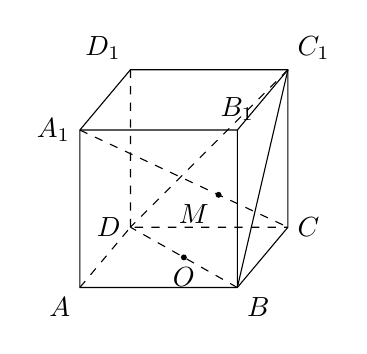
\begin{tikzpicture}[>=latex]
\draw (0,0) node [below left] {$A$} coordinate (A) --++ (2,0) node [below right] {$B$} coordinate (B) --++ (50:{2/2}) node [right] {$C$} coordinate (C)
--++ (0,2) node [above right] {$C_1$} coordinate (C1)
--++ (-2,0) node [above left] {$D_1$} coordinate (D1) --++ (230:{2/2}) node [left] {$A_1$} coordinate (A1) -- cycle;
\draw (A) ++ (2,2) node [above] {$B_1$} coordinate (B1) -- (B) (B1) --++ (50:{2/2}) (B1) --++ (-2,0);
\draw [dashed] (A) --++ (50:{2/2}) node [left] {$D$} coordinate (D) --++ (2,0) (D) --++ (0,2);
\draw (C1) -- (B);
\draw [dashed] (B) -- (D) (C1) -- (D) (A1) -- (C);
\filldraw ($(A1)!{2/3}!(C)$) circle (0.03) node [below left] {$M$} coordinate (M);
\filldraw ($(B)!0.5!(D)$) circle (0.03) node [below] {$O$} coordinate (O);
\end{tikzpicture}
\end{center}
\item 如图, 已知$A\in l$, $B\in l$, $C\in l$, $O\not\in l$. 求证: $OA$、$OB$、$OC$在同一平面上.
\begin{center}
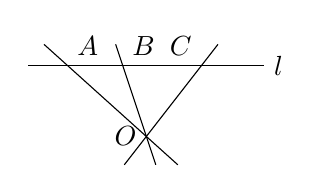
\begin{tikzpicture}[>=latex]
\draw (0,0) -- (3,0) node [right] {$l$};
\draw (0.5,0) node [above right] {$A$} coordinate (A);
\draw (1.2,0) node [above right] {$B$} coordinate (B);
\draw (2.2,0) node [above left] {$C$} coordinate (C);
\draw (1.5,-0.9) node [left] {$O$} coordinate (O);
\draw ($(O)!-0.4!(A)$) -- ($(O)!1.3!(A)$);
\draw ($(O)!-0.4!(B)$) -- ($(O)!1.3!(B)$);
\draw ($(O)!-0.4!(C)$) -- ($(O)!1.3!(C)$);
\end{tikzpicture}
\end{center}
\item 如图, 已知$D$及$E$是$\triangle ABC$的边$AC$及$BC$上的点, 平面$\alpha$经过$D$、$E$两点, 直线$AB$与平面$\alpha$交于点$P$. 求证:点$P$在直线$DE$上.
\begin{center}
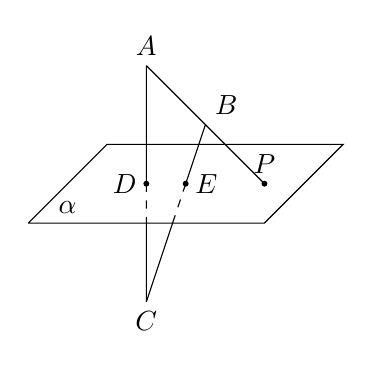
\begin{tikzpicture}[>=latex]
\draw [name path = plane] (0,0) -- (3,0) -- (4,1) -- (1,1) -- (0,0) ++ (0.5,0) node [above] {$\alpha$};
\filldraw (1.5,0.5) circle (0.03) node [left] {$D$} coordinate (D);
\filldraw (3,0.5) circle (0.03) node [above] {$P$} coordinate (P);
\filldraw (2,0.5) circle (0.03) node [right] {$E$} coordinate (E);
\draw (1.5,2) node [above] {$A$} coordinate (A);
\draw ($(A)!0.5!(P)$) node [above right] {$B$} coordinate (B);
\draw (A) -- (P) (B) -- (E) (A) -- (D);
\draw ($(A)!2!(D)$) node [below] {$C$} coordinate (C);
\path [name path = DC] (D) -- (C);
\path [name path = EC] (E) -- (C);
\path [name intersections = {of = DC and plane, by = S}];
\path [name intersections = {of = EC and plane, by = T}];
\draw (S) -- (C) (T) -- (C);
\draw [dashed] (D) -- (S) (E) -- (T);
\end{tikzpicture}
\end{center}
\item 如图, 已知$E$、$F$、$G$、$H$分别是正方体$ABCD-A_1B_1C_1D_1$的棱$AB$、$BC$、$CC_1$、$C_1D_1$的中点, 且$EF$与$HG$相交于点$Q$. 求证:点$Q$在直线$DC$上.
\begin{center}
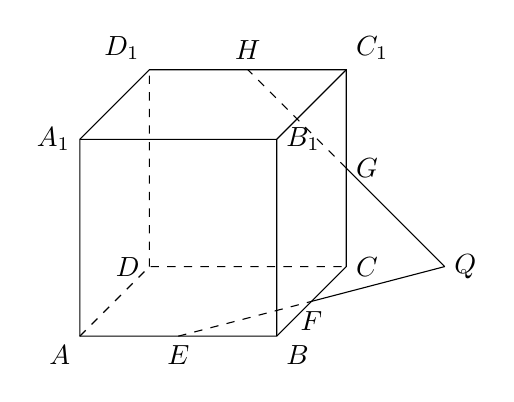
\begin{tikzpicture}[>=latex]
\draw (0,0) node [below left] {$A$} coordinate (A) --++ (2.5,0) node [below right] {$B$} coordinate (B) --++ (45:{2.5/2}) node [right] {$C$} coordinate (C)
--++ (0,2.5) node [above right] {$C_1$} coordinate (C1)
--++ (-2.5,0) node [above left] {$D_1$} coordinate (D1) --++ (225:{2.5/2}) node [left] {$A_1$} coordinate (A1) -- cycle;
\draw (A) ++ (2.5,2.5) node [right] {$B_1$} coordinate (B1) -- (B) (B1) --++ (45:{2.5/2}) (B1) --++ (-2.5,0);
\draw [dashed] (A) --++ (45:{2.5/2}) node [left] {$D$} coordinate (D) --++ (2.5,0) (D) --++ (0,2.5);
\draw ($(D)!1.5!(C)$) node [right] {$Q$} coordinate (Q);
\draw ($(A)!0.5!(B)$) node [below] {$E$} coordinate (E);
\draw ($(C)!0.5!(B)$) node [below] {$F$} coordinate (F);
\draw ($(C)!0.5!(C1)$) node [right] {$G$} coordinate (G);
\draw ($(C1)!0.5!(D1)$) node [above] {$H$} coordinate (H);
\draw [dashed] (E) -- (F) (G) -- (H);
\draw (F) -- (Q) (Q) -- (G);
\end{tikzpicture}
\end{center}




\iffalse



123



\fi


\begin{center}
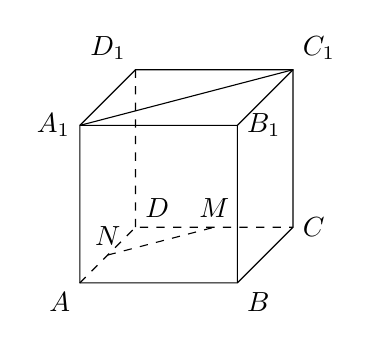
\begin{tikzpicture}[>=latex]
\draw (0,0) node [below left] {$A$} coordinate (A) --++ (2,0) node [below right] {$B$} coordinate (B) --++ (45:{2/2}) node [right] {$C$} coordinate (C)
--++ (0,2) node [above right] {$C_1$} coordinate (C1)
--++ (-2,0) node [above left] {$D_1$} coordinate (D1) --++ (225:{2/2}) node [left] {$A_1$} coordinate (A1) -- cycle;
\draw (A) ++ (2,2) node [right] {$B_1$} coordinate (B1) -- (B) (B1) --++ (45:{2/2}) (B1) --++ (-2,0);
\draw [dashed] (A) --++ (45:{2/2}) node [above right] {$D$} coordinate (D) --++ (2,0) (D) --++ (0,2);
\draw ($(A)!0.5!(D)$) node [above] {$N$} coordinate (N);
\draw ($(C)!0.5!(D)$) node [above] {$M$} coordinate (M);
\draw (A1) -- (C1);
\draw [dashed] (N) -- (M);
\end{tikzpicture}
\end{center}

\begin{center}
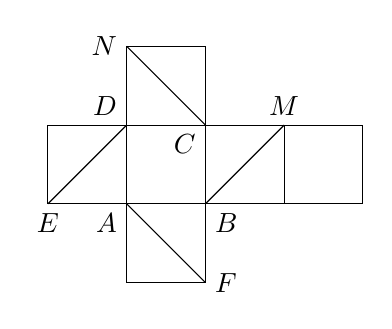
\begin{tikzpicture}[>=latex]
\draw (0,0) node [below] {$E$} rectangle (4,1);
\draw (1,2) node [left] {$N$} rectangle (2,-1) node [right] {$F$};
\draw (3,0) -- (3,1) node [above] {$M$};
\draw (2,0) node [below right] {$B$} -- (3,1);
\draw (1,0) node [below left] {$A$} -- (2,-1);
\draw (0,0) -- (1,1) node [above left] {$D$};
\draw (1,2) -- (2,1) node [below left] {$C$};
\end{tikzpicture}
\end{center}

\begin{center}
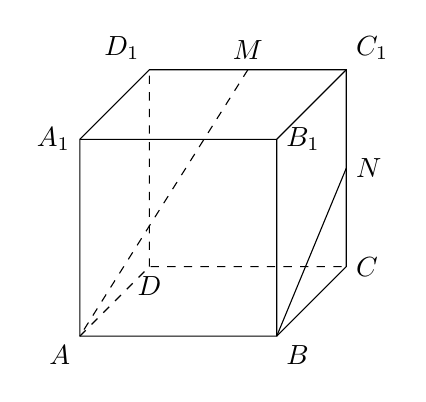
\begin{tikzpicture}[>=latex]
\draw (0,0) node [below left] {$A$} coordinate (A) --++ (2.5,0) node [below right] {$B$} coordinate (B) --++ (45:{2.5/2}) node [right] {$C$} coordinate (C)
--++ (0,2.5) node [above right] {$C_1$} coordinate (C1)
--++ (-2.5,0) node [above left] {$D_1$} coordinate (D1) --++ (225:{2.5/2}) node [left] {$A_1$} coordinate (A1) -- cycle;
\draw (A) ++ (2.5,2.5) node [right] {$B_1$} coordinate (B1) -- (B) (B1) --++ (45:{2.5/2}) (B1) --++ (-2.5,0);
\draw [dashed] (A) --++ (45:{2.5/2}) node [below] {$D$} coordinate (D) --++ (2.5,0) (D) --++ (0,2.5);
\draw ($(C)!0.5!(C1)$) node [right] {$N$} coordinate (N) -- (B);
\draw [dashed] ($(C1)!0.5!(D1)$) node [above] {$M$} coordinate (M) -- (A);
\end{tikzpicture}
\end{center}

\begin{center}
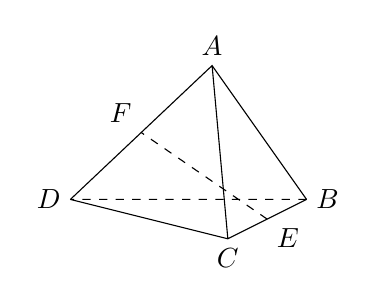
\begin{tikzpicture}[>=latex]
\draw (0,0) node [left] {$D$} coordinate (D);
\draw (3,0) node [right] {$B$} coordinate (B);
\draw (1.8,1.7) node [above] {$A$} coordinate (A);
\draw (2,-0.5) node [below] {$C$} coordinate (C);
\draw ($(B)!0.5!(C)$) node [below right] {$E$} coordinate (E);
\draw ($(A)!0.5!(D)$) node [above left] {$F$} coordinate (F);
\draw (A) -- (C) (B) -- (C) -- (D) (D) -- (A) -- (B);
\draw [dashed] (E) -- (F) (B) -- (D);
\end{tikzpicture}
\end{center}

\begin{center}
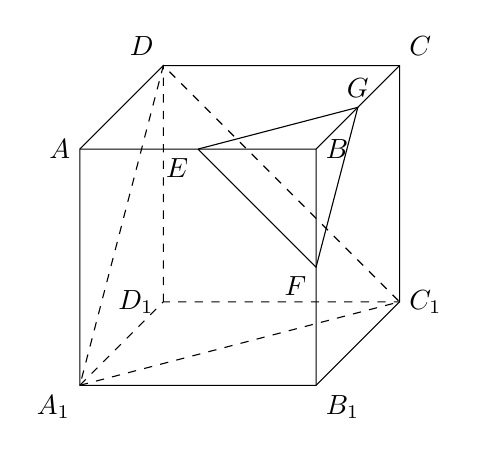
\begin{tikzpicture}[>=latex]
\draw (0,0) node [below left] {$A_1$} coordinate (A) --++ (3,0) node [below right] {$B_1$} coordinate (B) --++ (45:{3/2}) node [right] {$C_1$} coordinate (C)
--++ (0,3) node [above right] {$C$} coordinate (C1)
--++ (-3,0) node [above left] {$D$} coordinate (D1) --++ (225:{3/2}) node [left] {$A$} coordinate (A1) -- cycle;
\draw (A) ++ (3,3) node [right] {$B$} coordinate (B1) -- (B) (B1) --++ (45:{3/2}) (B1) --++ (-3,0);
\draw [dashed] (A) --++ (45:{3/2}) node [left] {$D_1$} coordinate (D) --++ (3,0) (D) --++ (0,3);
\draw [dashed] (A) -- (C) -- (D1) -- (A);
\draw ($(A1)!0.5!(B1)$) node [below left] {$E$} coordinate (E);
\draw ($(B1)!0.5!(B)$) node [below left] {$F$} coordinate (F);
\draw ($(B1)!0.5!(C1)$) node [above] {$G$} coordinate (G);
\draw (E) -- (F) -- (G) -- (E);
\end{tikzpicture}
\end{center}

\begin{center}
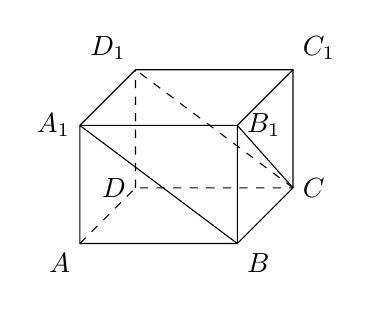
\begin{tikzpicture}[>=latex]
\draw (0,0) node [below left] {$A$} coordinate (A) --++ (2,0) node [below right] {$B$} coordinate (B) --++ (45:{2/2}) node [right] {$C$} coordinate (C)
--++ (0,1.5) node [above right] {$C_1$} coordinate (C1)
--++ (-2,0) node [above left] {$D_1$} coordinate (D1) --++ (225:{2/2}) node [left] {$A_1$} coordinate (A1) -- cycle;
\draw (A) ++ (2,1.5) node [right] {$B_1$} coordinate (B1) -- (B) (B1) --++ (45:{2/2}) (B1) --++ (-2,0);
\draw [dashed] (A) --++ (45:{2/2}) node [left] {$D$} coordinate (D) --++ (2,0) (D) --++ (0,1.5);
\draw (A1) -- (B) (B1) -- (C);
\draw [dashed] (C) -- (D1);
\end{tikzpicture}
\end{center}

\begin{center}
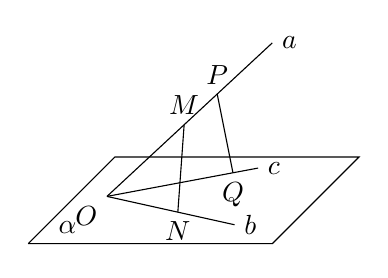
\begin{tikzpicture}[>=latex]
\draw (0.3,0.6) --++ (3.1,0) --++ (1.1,1.1) --++ (-3.1,0) -- (0.3,0.6) ++ (0.5,0) node [above] {$\alpha$};
\draw (1.3,1.2) node [below left] {$O$} coordinate (O);
\draw (2.7,2.5) node [above] {$P$} coordinate (P);
\draw ($(O)!0.7!(P)$) node [above] {$M$} coordinate (M);
\draw (O) -- ($(O)!1.5!(P)$) node [right] {$a$} coordinate (a);
\draw (2.2,1) node [below] {$N$} coordinate (N);
\draw (2.9,1.5) node [below] {$Q$} coordinate (Q);
\draw (O) -- ($(O)!1.8!(N)$) node [right] {$b$} coordinate (b);
\draw (O) -- ($(O)!1.2!(Q)$) node [right] {$c$} coordinate (c);
\draw (M) -- (N) (P) -- (Q);
\end{tikzpicture}
\end{center}

\begin{center}
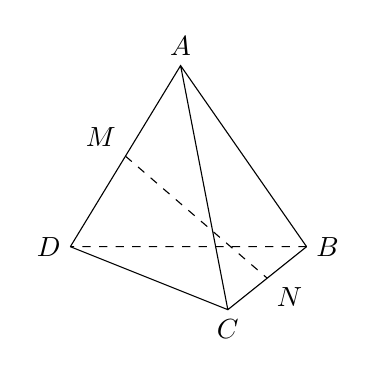
\begin{tikzpicture}[>=latex]
\draw (0,0) node [left] {$D$} coordinate (D);
\draw (3,0) node [right] {$B$} coordinate (B);
\draw (1.4,2.3) node [above] {$A$} coordinate (A);
\draw (2,-0.8) node [below] {$C$} coordinate (C);
\draw ($(B)!0.5!(C)$) node [below right] {$N$} coordinate (N);
\draw ($(A)!0.5!(D)$) node [above left] {$M$} coordinate (M);
\draw (A) -- (C) (B) -- (C) -- (D) (D) -- (A) -- (B);
\draw [dashed] (M) -- (N) (B) -- (D);
\end{tikzpicture}
\end{center}

\begin{center}
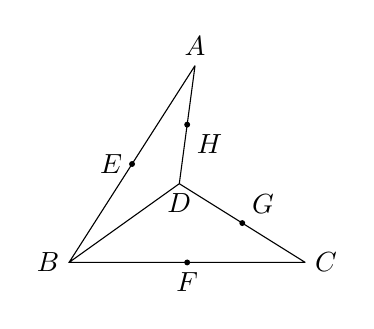
\begin{tikzpicture}[>=latex]
\draw (0,0) node [left] {$B$} coordinate (B);
\draw (3,0) node [right] {$C$} coordinate (C);
\draw (1.4,1) node [below] {$D$} coordinate (D);
\draw (1.6,2.5) node [above] {$A$} coordinate (A);
\filldraw ($(A)!0.5!(B)$) circle (0.03) node [left] {$E$} coordinate (E);
\filldraw ($(B)!0.5!(C)$) circle (0.03) node [below] {$F$} coordinate (F);
\filldraw ($(C)!0.5!(D)$) circle (0.03) node [above right] {$G$} coordinate (G);
\filldraw ($(D)!0.5!(A)$) circle (0.03) node [below right] {$H$} coordinate (H);
\draw (A) -- (B) -- (C) (A) -- (D) -- (C) (B) -- (D);
\end{tikzpicture}
\end{center}

\begin{center}
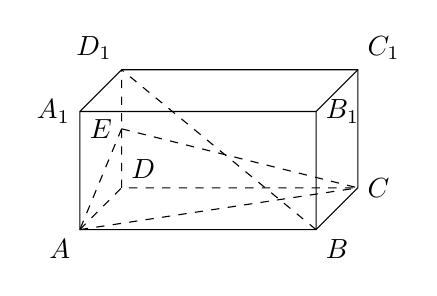
\begin{tikzpicture}[>=latex]
\draw (0,0) node [below left] {$A$} coordinate (A) --++ (3,0) node [below right] {$B$} coordinate (B) --++ (45:{1.5/2}) node [right] {$C$} coordinate (C)
--++ (0,1.5) node [above right] {$C_1$} coordinate (C1)
--++ (-3,0) node [above left] {$D_1$} coordinate (D1) --++ (225:{1.5/2}) node [left] {$A_1$} coordinate (A1) -- cycle;
\draw (A) ++ (3,1.5) node [right] {$B_1$} coordinate (B1) -- (B) (B1) --++ (45:{1.5/2}) (B1) --++ (-3,0);
\draw [dashed] (A) --++ (45:{1.5/2}) node [above right] {$D$} coordinate (D) --++ (3,0) (D) --++ (0,1.5);
\draw [dashed] (B) -- (D1);
\draw ($(D)!0.5!(D1)$) node [left] {$E$} coordinate (E);
\draw [dashed] (E) -- (A) (E) -- (C) (A) -- (C);
\end{tikzpicture}
\end{center}

\begin{center}
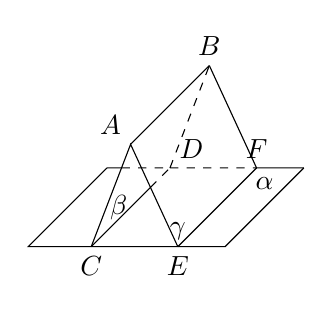
\begin{tikzpicture}[>=latex]
\path [name path = plane]  (1,1) --++ (2.5,0);
\draw (1,1) -- (0,0) -- (2.5,0) --++ (1,1);
\draw (0.8,0) node [below] {$C$} coordinate (C);
\draw (1.9,0) node [below] {$E$} coordinate (E);
\draw (1.3,1.3) node [above left] {$A$} coordinate (A);
\draw (C) -- (A) -- (E);
\draw (A) --++ (1,1) node [above] {$B$} coordinate (B);
\draw (E) --++ (1,1) node [above] {$F$} coordinate (F);
\path [name path = CD] (C) --++ (1,1) node [above right] {$D$}coordinate (D);
\path [name path = CA] (C) -- (A);
\path [name path = EA] (E) -- (A);
\draw (B) -- (F) -- (3.5,1);
\draw [dashed] (D) -- (B) (D) -- (F);
\path [name intersections = {of = CA and plane, by = S}];
\path [name intersections = {of = CD and EA, by = T}];
\draw (S) -- (1,1) (C) -- (T);
\draw [dashed] (S) -- (D) (T) -- (D);
\draw (C) ++ (0.35,0.5) node {$\beta$};
\draw (E) ++ (0,0.2) node {$\gamma$};
\draw (3,1) node [below] {$\alpha$};
\end{tikzpicture}
\end{center}

\begin{center}
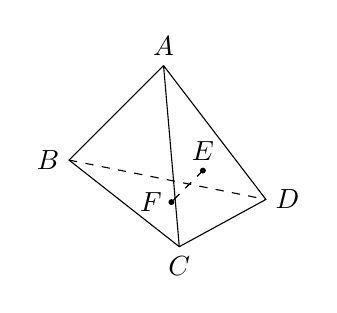
\begin{tikzpicture}[>=latex]
\draw (0,0) node [left] {$B$} coordinate (B);
\draw (2.5,-0.5) node [right] {$D$} coordinate (D);
\draw (1.2,1.2) node [above] {$A$} coordinate (A);
\draw (1.4,-1.1) node [below] {$C$} coordinate (C);
\filldraw ($(B)!{2/3}!($(C)!0.5!(D)$)$) circle (0.03) node [left]  {$F$} coordinate (F);
\filldraw ($(C)!{2/3}!($(A)!0.5!(D)$)$) circle (0.03) node [above]  {$E$} coordinate (E);
\draw (A) -- (B) -- (C) -- (D) -- (A) (A) -- (C);
\draw [dashed] (B) -- (D) (E) -- (F);
\end{tikzpicture}
\end{center}


\begin{center}
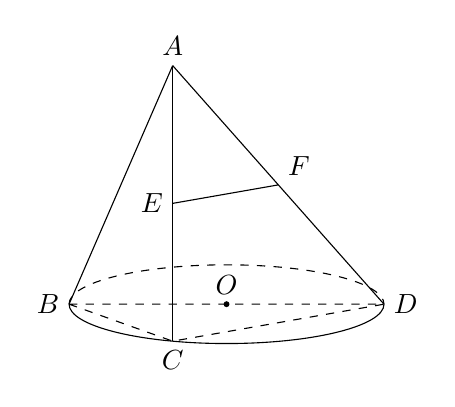
\begin{tikzpicture}[>=latex]
\filldraw (0,0) circle (0.03) node [above] {$O$} coordinate (O);
\draw (-2,0) node [left] {$B$} coordinate (B) arc (180:360:2 and 0.5) node [right] {$D$} coordinate (D);
\draw [dashed] (-2,0) arc (180:0:2 and 0.5);
\draw ({2*cos(250)},{0.5*sin(250)}) node [below] {$C$} coordinate (C) --++ (0,3.5) node [above] {$A$} coordinate (A);
\draw ($(A)!0.5!(C)$) node [left] {$E$} coordinate (E);
\draw ($(A)!0.5!(D)$) node [above right] {$F$} coordinate (F);
\draw (A) -- (B) (A) -- (D) (E) -- (F);
\draw [dashed] (B) -- (D) (B) -- (C) -- (D);
\end{tikzpicture}
\end{center}

\begin{center}
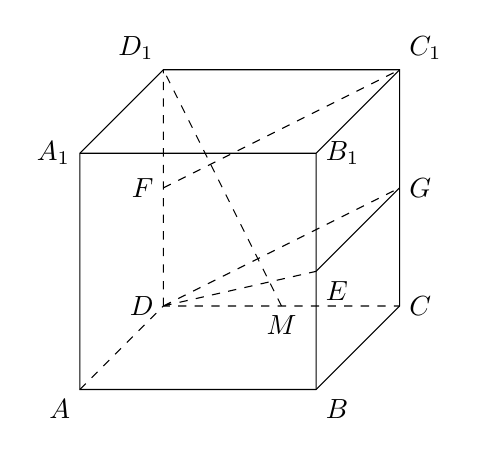
\begin{tikzpicture}[>=latex]
\draw (0,0) node [below left] {$A$} coordinate (A) --++ (3,0) node [below right] {$B$} coordinate (B) --++ (45:{3/2}) node [right] {$C$} coordinate (C)
--++ (0,3) node [above right] {$C_1$} coordinate (C1)
--++ (-3,0) node [above left] {$D_1$} coordinate (D1) --++ (225:{3/2}) node [left] {$A_1$} coordinate (A1) -- cycle;
\draw (A) ++ (3,3) node [right] {$B_1$} coordinate (B1) -- (B) (B1) --++ (45:{3/2}) (B1) --++ (-3,0);
\draw [dashed] (A) --++ (45:{3/2}) node [left] {$D$} coordinate (D) --++ (3,0) (D) --++ (0,3);
\draw ($(B)!0.5!(B1)$)node [below right] {$E$} coordinate (E) -- ($(C)!0.5!(C1)$) node [right] {$G$} coordinate (G);
\draw [dashed] (D) -- (E) (D) -- (G);
\draw [dashed] ($(D)!0.5!(D1)$) node [left] {$F$} coordinate (F) -- (C1);
\draw [dashed] ($(C)!0.5!(D)$) node [below] {$M$} coordinate (M) -- (D1);
\end{tikzpicture}
\end{center}

\begin{center}
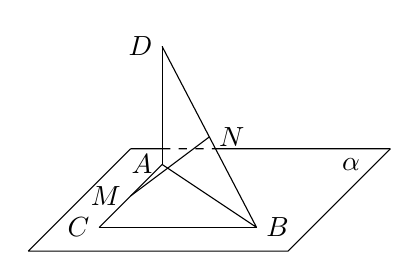
\begin{tikzpicture}[>=latex]
\draw (0,0) node [left] {$C$} coordinate (C) -- (2,0) node [right] {$B$} coordinate (B);
\draw (0.8,0.8) node [left] {$A$} coordinate (A) --++ (0,1.5) node [left] {$D$} coordinate (D);
\draw (A) -- (C) (A) -- (B) (B) -- (D);
\draw ($(A)!0.5!(C)$) node [left] {$M$} coordinate (M);
\draw ($(B)!0.5!(D)$) node [right] {$N$} coordinate (N);
\draw (M) -- (N);
\draw (-0.9,-0.3) --++ (3.3,0) --++ (1.3,1.3) coordinate (R) ++ (-3.3,0) coordinate (P) --++ (-1.3,-1.3);
\path [name path = rear] (R) --++ (-3.3,0);
\path [name path = BD] (B) -- (D);
\path [name path = AD] (A) -- (D);
\path [name intersections = {of = AD and rear, by = S}];
\path [name intersections = {of = BD and rear, by = T}];
\draw (S) -- (P) (T) -- (R);
\draw [dashed] (S) -- (T);
\draw (R) ++ (-0.5,0) node [below] {$\alpha$};
\end{tikzpicture}
\end{center}

\begin{center}
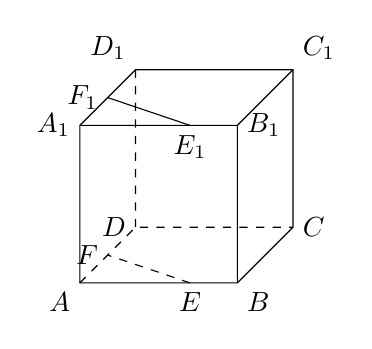
\begin{tikzpicture}[>=latex]
\draw (0,0) node [below left] {$A$} coordinate (A) --++ (2,0) node [below right] {$B$} coordinate (B) --++ (45:{2/2}) node [right] {$C$} coordinate (C)
--++ (0,2) node [above right] {$C_1$} coordinate (C1)
--++ (-2,0) node [above left] {$D_1$} coordinate (D1) --++ (225:{2/2}) node [left] {$A_1$} coordinate (A1) -- cycle;
\draw (A) ++ (2,2) node [right] {$B_1$} coordinate (B1) -- (B) (B1) --++ (45:{2/2}) (B1) --++ (-2,0);
\draw [dashed] (A) --++ (45:{2/2}) node [left] {$D$} coordinate (D) --++ (2,0) (D) --++ (0,2);
\draw ($(A)!0.7!(B)$) node [below] {$E$} coordinate (E);
\draw ($(A1)!0.7!(B1)$) node [below] {$E_1$} coordinate (E1);
\draw ($(A)!0.5!(D)$) node [left] {$F$} coordinate (F);
\draw ($(A1)!0.5!(D1)$) node [left] {$F_1$} coordinate (F1);
\draw (E1) -- (F1);
\draw [dashed] (E) -- (F);
\end{tikzpicture}
\end{center}

\begin{center}
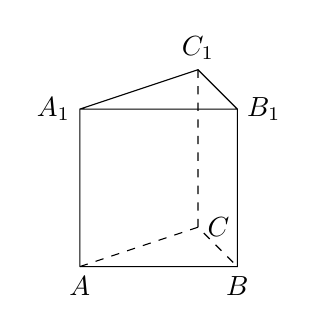
\begin{tikzpicture}[>=latex]
\draw (0,0) node [below] {$A$} coordinate (A);
\draw (2,0) node [below] {$B$} coordinate (B);
\draw (1.5,0.5) node [right] {$C$} coordinate (C);
\draw (A) ++ (0,2) node [left] {$A_1$} coordinate (A1);
\draw (B) ++ (0,2) node [right] {$B_1$} coordinate (B1);
\draw (C) ++ (0,2) node [above] {$C_1$} coordinate (C1);
\draw (A) -- (B) -- (B1) -- (A1) -- (A) (A1) -- (C1) -- (B1);
\draw [dashed] (A) -- (C) -- (B) (C) -- (C1);
\end{tikzpicture}
\end{center}

\begin{center}
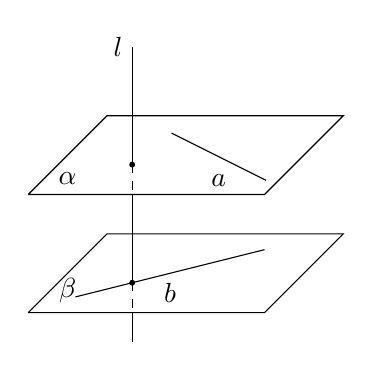
\begin{tikzpicture}[>=latex]
\draw (0,0) --++ (3,0) --++ (1,1) --++ (-3,0) --++ (-1,-1) coordinate (beta);
\draw (0,1.5) --++ (3,0) --++ (1,1) --++ (-3,0) --++ (-1,-1) coordinate (alpha);
\draw (alpha) ++ (0.5,0) node [above] {$\alpha$} (beta) ++ (0.5,0) node [above] {$\beta$};
\draw (0.6,0.2) coordinate (A) -- (3,0.8) coordinate (B);
\filldraw ($(A)!0.3!(B)$) circle (0.03) coordinate (C);
\filldraw (C) ++ (0,1.5) circle (0.03) coordinate (D);
\path [name path = CD] ($(C)!2!(D)$) -- ($(C)!-0.5!(D)$);
\path [name path = aboveline] (0,1.5) --++ (3,0);
\path [name path = belowline] (0,0) --++ (3,0);
\path [name intersections = {of = CD and aboveline, by = D1}];
\path [name intersections = {of = CD and belowline, by = C1}];
\draw ($(C)!2!(D)$) node [left] {$l$} -- (D) (D1) -- (C) (C1) -- ($(C)!-0.5!(D)$);
\draw [dashed] (D) -- (D1) (C) -- (C1);
\draw (D) ++ (0.5,0.4) --++ (1.2,-0.6);
\draw (D) ++ (1.1,0) node [below] {$a$};
\draw ($(A)!0.5!(B)$) node [below] {$b$};
\end{tikzpicture}
\end{center}

\begin{center}
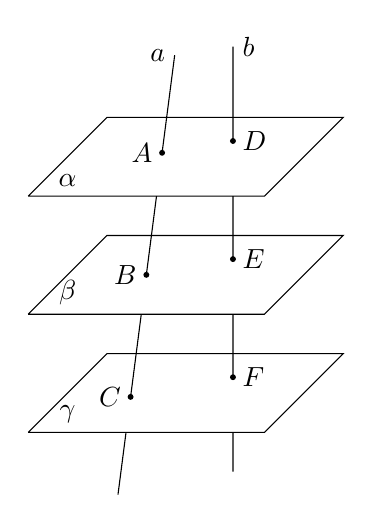
\begin{tikzpicture}[>=latex]
\draw (0,0) --++ (3,0) --++ (1,1) --++ (-3,0) --++ (-1,-1) ++ (0.5,0) node [above] {$\gamma$};
\draw (0,1.5) --++ (3,0) --++ (1,1) --++ (-3,0) --++ (-1,-1) ++ (0.5,0) node [above] {$\beta$};
\draw (0,3) --++ (3,0) --++ (1,1) --++ (-3,0) --++ (-1,-1) ++ (0.5,0) node [above] {$\alpha$};
\filldraw (2.6,2.2) circle (0.03) node [right] {$E$} coordinate (E);
\filldraw (1.5,2) circle (0.03) node [left] {$B$} coordinate (B);
\filldraw (E) ++ (0,1.5) circle (0.03) node [right] {$D$} coordinate (D);
\filldraw (E) ++ (0,-1.5) circle (0.03) node [right] {$F$} coordinate (F);
\filldraw (B) ++ (0.2,1.55) circle (0.03) node [left] {$A$} coordinate (A);
\filldraw (B) ++ (-0.2,-1.55) circle (0.03) node [left] {$C$} coordinate (C);
\path [name path = AC] ($(A)!-0.4!(C)$) node [left] {$a$} -- ($(A)!1.4!(C)$);
\path [name path = DF] ($(D)!-0.4!(F)$) node [right] {$b$} -- ($(D)!1.4!(F)$);
\path [name path = line1] (0,3) --++ (3,0);
\path [name path = line2] (0,1.5) --++ (3,0);
\path [name path = line3] (0,0) --++ (3,0);
\path [name intersections = {of = line1 and AC, by = A1}];
\path [name intersections = {of = line2 and AC, by = B1}];
\path [name intersections = {of = line3 and AC, by = C1}];
\path [name intersections = {of = line1 and DF, by = D1}];
\path [name intersections = {of = line2 and DF, by = E1}];
\path [name intersections = {of = line3 and DF, by = F1}];
\draw ($(A)!-0.4!(C)$) -- (A) (A1) -- (B) (B1) -- (C) (C1) -- ($(A)!1.4!(C)$);
\draw ($(D)!-0.4!(F)$) -- (D) (D1) -- (E) (E1) -- (F) (F1) -- ($(D)!1.4!(F)$);
\end{tikzpicture}
\end{center}

\begin{center}
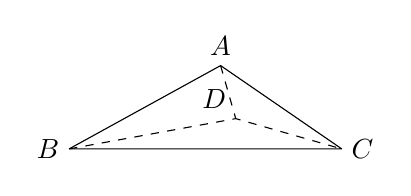
\begin{tikzpicture}[>=latex]
\draw ({sqrt(3)},0,0) node [right] {$C$} coordinate (C);
\draw ({-sqrt(3)},0,0) node [left] {$B$} coordinate (B);
\draw (0,0,-1) node [above left] {$D$} coordinate (D);
\draw (0,{sqrt(3)/2},{-1/2}) node [above] {$A$} coordinate (A);
\draw (B) -- (C) (B) -- (A) -- (C);
\draw [dashed] (A) -- (D) (B) -- (D) -- (C);
\end{tikzpicture}
\end{center}

\begin{center}
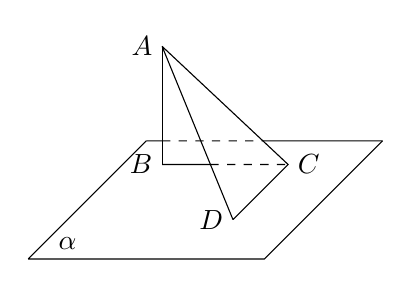
\begin{tikzpicture}[>=latex]
\draw (0,0) --++ (3,0) --++ (1.5,1.5) ++ (-3,0) --++ (-1.5,-1.5) ++ (0.5,0) node [above] {$\alpha$};
\draw (1.7,1.2) node [left] {$B$} coordinate (B) --++ (0,1.5) node [left] {$A$} coordinate (A);
\draw (B) ++ (1.6,0) node [right] {$C$} coordinate (C);
\draw (C) ++ (-0.7,-0.7) node [left] {$D$} coordinate (D);
\draw (A) -- (C) -- (D) (A) -- (D);
\path [name path = AD] (A) -- (D);
\path [name path = BC] (B) -- (C);
\path [name path = AB] (A) -- (B);
\path [name path = AC] (A) -- (C);
\path [name path = line] (1.5,1.5) --++ (3,0);
\path [name intersections = {of = AB and line, by = P}];
\path [name intersections = {of = AC and line, by = Q}];
\path [name intersections = {of = AD and BC, by = T}];
\draw (1.5,1.5) -- (P) (Q) -- (4.5,1.5) (B) -- (T);
\draw [dashed] (P) -- (Q) (T) -- (C);
\end{tikzpicture}
\end{center}

\begin{center}
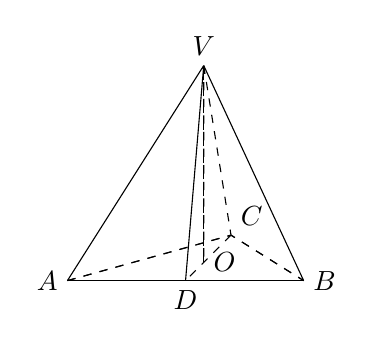
\begin{tikzpicture}[>=latex]
\draw (-1.5,0,0) node [left] {$A$} coordinate (A) -- (1.5,0,0) node [right] {$B$} coordinate (B);
\draw (0,0,0) node [below] {$D$} coordinate (D);
\draw (0,0,-1.5) node [above right] {$C$} coordinate (C);
\draw [dashed] (C) -- (D) (A) -- (C) -- (B);
\draw ($(D)!0.4!(C)$) node [right] {$O$} coordinate (O);
\draw [dashed] (O) --++ (0,2.5,0) node [above] {$V$} coordinate (V);
\draw (V) -- (A) (V) -- (B) (V) -- (D);
\draw [dashed] (V) -- (O) (V) -- (C) (A) -- (C) -- (B); 
\end{tikzpicture}
\end{center}

\begin{center}
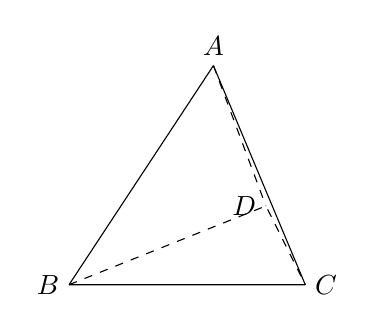
\begin{tikzpicture}[>=latex]
\draw (0,0,0) node [left] {$B$} coordinate (B);
\draw (3,0,0) node [right] {$C$} coordinate (C);
\draw (1.5,0,0) ++ (0,0,{-1.5*sqrt(3)}) node [left] {$D$} coordinate (D);
\draw (1.5,0,0) ++ (0,0,{-0.5*sqrt(3)}) ++ (0,{sqrt(6)},0) node [above] {$A$} coordinate (A); 
\draw (A) -- (B) (A) -- (C) (B) -- (C);
\draw [dashed] (B) -- (D) -- (C) (A) -- (D);
\end{tikzpicture}
\end{center}

\begin{center}
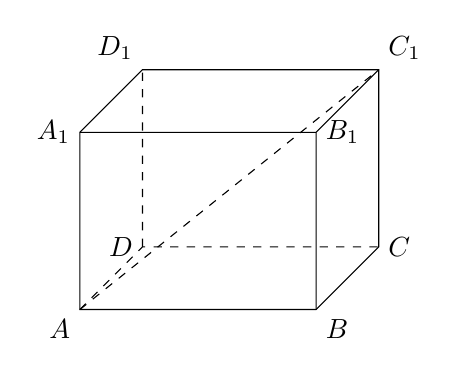
\begin{tikzpicture}[>=latex,scale = 1.5]
\draw (0,0) node [below left] {$A$} coordinate (A) --++ (2,0) node [below right] {$B$} coordinate (B) --++ (45:{1.5/2}) node [right] {$C$} coordinate (C)
--++ (0,1.5) node [above right] {$C_1$} coordinate (C1)
--++ (-2,0) node [above left] {$D_1$} coordinate (D1) --++ (225:{1.5/2}) node [left] {$A_1$} coordinate (A1) -- cycle;
\draw (A) ++ (2,1.5) node [right] {$B_1$} coordinate (B1) -- (B) (B1) --++ (45:{1.5/2}) (B1) --++ (-2,0);
\draw [dashed] (A) --++ (45:{1.5/2}) node [left] {$D$} coordinate (D) --++ (2,0) (D) --++ (0,1.5);
\draw [dashed] (A) -- (C1);
\end{tikzpicture}
\end{center}

\begin{center}
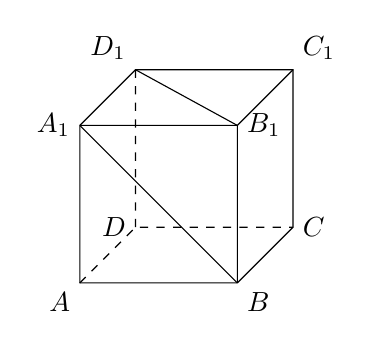
\begin{tikzpicture}[>=latex]
\draw (0,0) node [below left] {$A$} coordinate (A) --++ (2,0) node [below right] {$B$} coordinate (B) --++ (45:{2/2}) node [right] {$C$} coordinate (C)
--++ (0,2) node [above right] {$C_1$} coordinate (C1)
--++ (-2,0) node [above left] {$D_1$} coordinate (D1) --++ (225:{2/2}) node [left] {$A_1$} coordinate (A1) -- cycle;
\draw (A) ++ (2,2) node [right] {$B_1$} coordinate (B1) -- (B) (B1) --++ (45:{2/2}) (B1) --++ (-2,0);
\draw [dashed] (A) --++ (45:{2/2}) node [left] {$D$} coordinate (D) --++ (2,0) (D) --++ (0,2);
\draw (A1) -- (B) (B1) -- (D1);
\end{tikzpicture}
\end{center}

\begin{center}
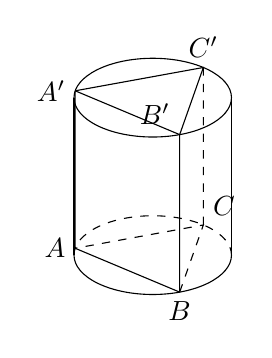
\begin{tikzpicture}[>=latex]
\draw (0,0) ellipse (1 and 0.5);
\draw (-1,-2) arc (180:360:1 and 0.5);
\draw [dashed] (-1,-2) arc (180:0:1 and 0.5);
\draw (0,-2) ++ ({cos(50)},{0.5*sin(50)}) node [above right] {$C$} coordinate (C);
\draw (0,-2) ++ ({cos(170)},{0.5*sin(170)}) node [left] {$A$} coordinate (A);
\draw (0,-2) ++ ({cos(290)},{0.5*sin(290)}) node [below] {$B$} coordinate (B);
\draw (A) ++ (0,2) node [left] {$A'$} coordinate (A1);
\draw (B) ++ (0,2) node [above left] {$B'$} coordinate (B1);
\draw (C) ++ (0,2) node [above] {$C'$} coordinate (C1);
\draw (A1) -- (B1) -- (C1) -- (A1);
\draw (A) -- (A1) (B) -- (B1) (A) -- (B);
\draw [dashed] (B) -- (C) -- (A) (C) -- (C1);
\draw (-1,-2) -- (-1,0) (1,-2) -- (1,0);
\end{tikzpicture}
\end{center}

\begin{center}
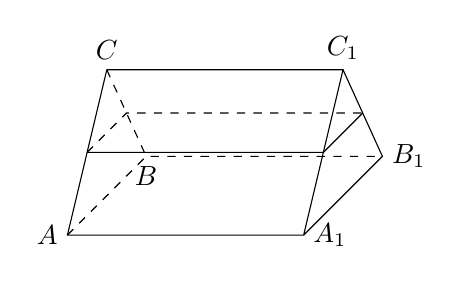
\begin{tikzpicture}[>=latex]
\draw (0,0) node [left] {$A$} coordinate (A);
\draw (1,1) node [below] {$B$} coordinate (B);
\draw (0.5,2.1) node [above] {$C$} coordinate (C);
\draw (A) ++ (3,0) node [right] {$A_1$} coordinate (A1);
\draw (B) ++ (3,0) node [right] {$B_1$} coordinate (B1);
\draw (C) ++ (3,0) node [above] {$C_1$} coordinate (C1);
\draw (C) -- (C1) -- (A1) -- (A) -- (C) (A1) -- (B1) -- (C1);
\draw [dashed] (C) -- (B) -- (B1) (A) -- (B);
\draw ($(A)!0.5!(C)$) --++ (3,0) --++ (0.5,0.5);
\draw [dashed] ($(A)!0.5!(C)$) --++ (0.5,0.5) --++ (3,0);
\end{tikzpicture}
\end{center}


\begin{center}
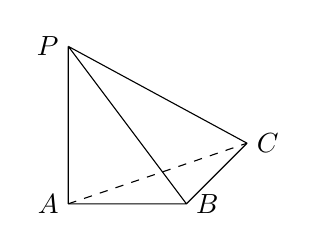
\begin{tikzpicture}[>=latex,scale = 0.5]
\draw (0,0,0) node [left] {$A$} coordinate (A);
\draw (A) ++ (0,4,0) node [left] {$P$} coordinate (P);
\draw (A) ++ (3,0,0) node [right] {$B$} coordinate (B);
\draw (B) ++ (0,0,-4) node [right] {$C$} coordinate (C);
\draw (A) -- (B) -- (C) (P) -- (A) (P) -- (C) (P) -- (B);
\draw [dashed] (A) -- (C);
\end{tikzpicture}
\end{center}

\begin{center}
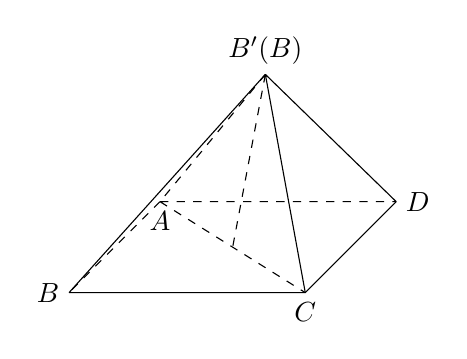
\begin{tikzpicture}[>=latex]
\draw (0,0,0) node [left] {$B$} coordinate (B);
\draw (3,0,0) node [below] {$C$} coordinate (C);
\draw (3,0,-3) node [right] {$D$} coordinate (D);
\draw (0,0,-3) node [below] {$A$} coordinate (A);
\draw (B) -- (C) -- (D);
\draw [dashed] (A) -- (B) (A) -- (C) (A) -- (D);
\draw (1.8,{sqrt(2*pow(1.5,2)-2*pow(0.3,2))},-1.8) node [above] {$B'(B)$} coordinate (B1);
\draw (B) -- (B1) (B1) -- (C) (B1) -- (D);
\draw [dashed] (B1) -- (A) (B1) -- ($(A)!0.5!(C)$);
\end{tikzpicture}
\end{center}

\begin{center}
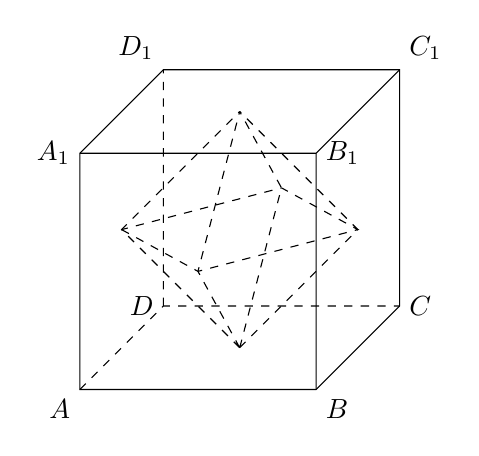
\begin{tikzpicture}[>=latex]
\draw (0,0) node [below left] {$A$} coordinate (A) --++ (3,0) node [below right] {$B$} coordinate (B) --++ (45:{3/2}) node [right] {$C$} coordinate (C)
--++ (0,3) node [above right] {$C_1$} coordinate (C1)
--++ (-3,0) node [above left] {$D_1$} coordinate (D1) --++ (225:{3/2}) node [left] {$A_1$} coordinate (A1) -- cycle;
\draw (A) ++ (3,3) node [right] {$B_1$} coordinate (B1) -- (B) (B1) --++ (45:{3/2}) (B1) --++ (-3,0);
\draw [dashed] (A) --++ (45:{3/2}) node [left] {$D$} coordinate (D) --++ (3,0) (D) --++ (0,3);
\draw ($(A)!0.5!(D1)$) coordinate (P);
\draw ($(B)!0.5!(A1)$) coordinate (Q);
\draw ($(C)!0.5!(B1)$) coordinate (R);
\draw ($(D)!0.5!(C1)$) coordinate (S);
\draw ($(A)!0.5!(C)$) coordinate (X);
\draw ($(A1)!0.5!(C1)$) coordinate (Y);
\draw [dashed] (P) -- (Q) -- (R) -- (S) -- (P);
\draw [dashed] (X) -- (P) -- (Y) (X) -- (Q) -- (Y) (X) -- (R) -- (Y) (X) -- (S) -- (Y);
\end{tikzpicture}
\end{center}

\begin{center}
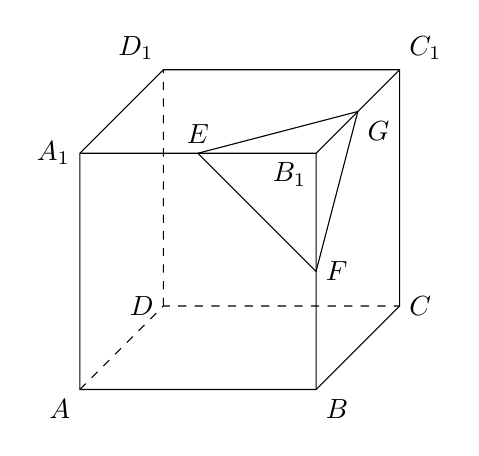
\begin{tikzpicture}[>=latex]
\draw (0,0) node [below left] {$A$} coordinate (A) --++ (3,0) node [below right] {$B$} coordinate (B) --++ (45:{3/2}) node [right] {$C$} coordinate (C)
--++ (0,3) node [above right] {$C_1$} coordinate (C1)
--++ (-3,0) node [above left] {$D_1$} coordinate (D1) --++ (225:{3/2}) node [left] {$A_1$} coordinate (A1) -- cycle;
\draw (A) ++ (3,3) node [below left] {$B_1$} coordinate (B1) -- (B) (B1) --++ (45:{3/2}) (B1) --++ (-3,0);
\draw [dashed] (A) --++ (45:{3/2}) node [left] {$D$} coordinate (D) --++ (3,0) (D) --++ (0,3);
\draw ($(B1)!0.5!(A1)$) node [above] {$E$} coordinate (E);
\draw ($(B)!0.5!(B1)$) node [right] {$F$} coordinate (F);
\draw ($(B1)!0.5!(C1)$) node [below right] {$G$} coordinate (G);
\draw (E) -- (F) -- (G) -- cycle;
\end{tikzpicture}
\end{center}

\begin{center}
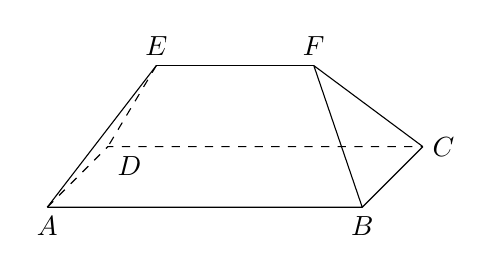
\begin{tikzpicture}[>=latex]
\draw (0,0,0) node [below] {$A$} coordinate (A);
\draw (4,0,0) node [below] {$B$} coordinate (B);
\draw (0,0,-2) node [below right] {$D$} coordinate (D);
\draw (4,0,-2) node [right] {$C$} coordinate (C);
\draw (1,{sqrt(2)},-1) node [above] {$E$} coordinate (E);
\draw (E) --++ (2,0,0) node [above] {$F$} coordinate (F);
\draw (A) -- (B) -- (C) (A) -- (E) (F) -- (B) (F) -- (C);
\draw [dashed] (E) -- (D) (A) -- (D) -- (C);
\end{tikzpicture}
\end{center}

\begin{center}
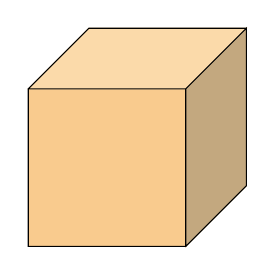
\begin{tikzpicture}[>=latex]
\definecolor{frontcolor}{RGB}{249, 203, 142}
\filldraw [frontcolor] (0,0,0) rectangle (2,2,0);
\definecolor{rightcolor}{RGB}{195, 168, 127}
\filldraw [rightcolor] (2,0,0)  -- (2,0,-2) -- (2,2,-2) -- (2,2,0) -- cycle;
\definecolor{abovecolor}{RGB}{251, 218, 170}
\filldraw [abovecolor] (0,2,0) -- (2,2,0) -- (2,2,-2) -- (0,2,-2) -- cycle;
\draw (0,0,0) rectangle (2,2,0) (2,0,0)  -- (2,0,-2) -- (2,2,-2) -- (2,2,0) (0,2,0) -- (0,2,-2) -- (2,2,-2);
\end{tikzpicture}
\end{center}

\begin{center}
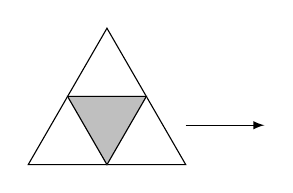
\begin{tikzpicture}[>=latex]
\draw (0,0) -- (2,0) -- (60:2) -- cycle;
\filldraw [gray!50] (60:1) --++ (1,0) -- (1,0) -- cycle;
\draw (60:1) --++ (1,0) -- (1,0) -- cycle;
\draw [->] (2,0.5) -- (3,0.5);
\end{tikzpicture}
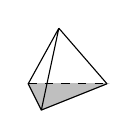
\begin{tikzpicture}[>=latex]
\draw (0,0,0) coordinate (A)  (1,0,0) coordinate (B)  (0.5,0,{0.5*sqrt(3)}) coordinate (C) (C) ++ (0,0,{-0.5*sqrt(3)/3*2}) ++ (0,{sqrt(6)/3},0) coordinate (D);
\filldraw [gray!50] (A) -- (C) -- (B) -- cycle;
\draw (D) -- (A) (D) -- (B) (D) -- (C) (A) -- (C) -- (B);
\draw [dashed] (A) -- (B);
\end{tikzpicture}
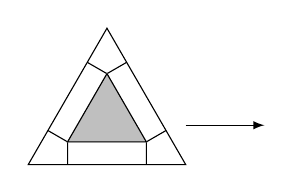
\begin{tikzpicture}[>=latex]
\draw (0,0) -- (2,0) -- (60:2) -- cycle;
\draw (30:{1/sqrt(3)}) coordinate (A);
\draw (A) ++ (1,0) coordinate (B);
\draw (A) ++ (60:1) coordinate (C);
\draw (A) --++ (0,{-0.5/sqrt(3)}) (A) --++ (150:{0.5/sqrt(3)});
\draw (B) --++ (270:{0.5/sqrt(3)}) (B) --++ (30:{0.5/sqrt(3)});
\draw (C) --++ (30:{0.5/sqrt(3)}) (C) --++ (150:{0.5/sqrt(3)});
\filldraw [gray!50] (A) -- (B) -- (C) -- cycle;
\draw (A) -- (B) -- (C) -- cycle;
\draw [->] (2,0.5) -- (3,0.5);
\end{tikzpicture}
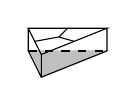
\begin{tikzpicture}[>=latex]
\draw (0,0,0) coordinate (A)  (1,0,0) coordinate (B)  (0.5,0,{0.5*sqrt(3)}) coordinate (C);
\filldraw [gray!50] (A) -- (C) -- (B) -- cycle;
\draw (A) ++ (0,{0.5/sqrt(3)}) coordinate (A1) (B) ++ (0,{0.5/sqrt(3)}) coordinate (B1) (C) ++ (0,{0.5/sqrt(3)}) coordinate (C1);
\draw (A1) -- (B1) -- (C1) -- cycle;
\draw (A) -- (A1) (B) -- (B1) (C) -- (C1) (A) -- (C) -- (B);
\draw [dashed] (A) -- (B);
\draw (C1) ++ (0,0,{-0.5*sqrt(3)/3*2}) coordinate (D);
\draw ($(A1)!0.5!(B1)$) -- (D) ($(C1)!0.5!(B1)$) -- (D) ($(C1)!0.5!(A1)$) -- (D);
\end{tikzpicture}
\end{center}

\begin{center}
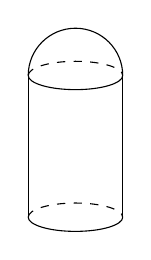
\begin{tikzpicture}[>=latex,scale = 0.6]
\draw (-1,0) arc (180:360:1 and 0.3);
\draw (-1,3) arc (180:360:1 and 0.3);
\draw [dashed] (-1,0) arc (180:0:1 and 0.3);
\draw [dashed] (-1,3) arc (180:0:1 and 0.3);
\draw (-1,3) arc (180:0:1);
\draw (-1,0) -- (-1,3) (1,0) -- (1,3);
\end{tikzpicture}
\end{center}

\begin{center}
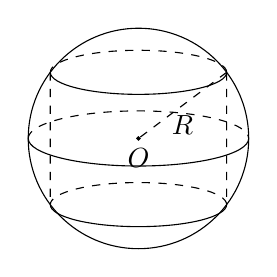
\begin{tikzpicture}[>=latex,scale = 0.7]
\draw (0,0) circle (2);
\filldraw (0,0) circle (0.03) node [below] {$O$} coordinate (O);
\draw [dashed] (1.6,1.2) coordinate (P) -- (O);
\draw (-2,0) arc (180:360:2 and 0.5);
\draw (0.8,0.6) node [below] {$R$};
\draw [dashed] (-2,0) arc (180:0:2 and 0.5);
\draw [dashed] (P) -- (1.6,-1.2) (-1.6,1.2) -- (-1.6,-1.2);
\draw (P) arc (0:-180:1.6 and 0.4);
\draw (P) ++ (0,-2.4) arc (0:-180:1.6 and 0.4);
\draw [dashed] (P) arc (0:180:1.6 and 0.4);
\draw [dashed] (P) ++ (0,-2.4) arc (0:180:1.6 and 0.4);
\end{tikzpicture}
\end{center}

以下是选择性必修一, 暂借这里.

\begin{center}
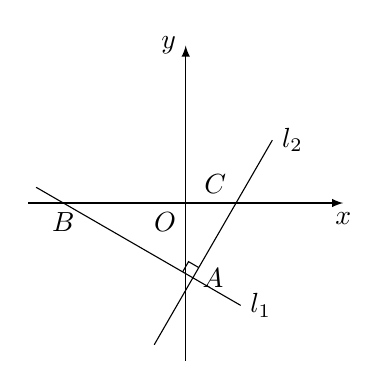
\begin{tikzpicture}[>=latex]
\draw [->, name path = x] (-2,0) -- (2,0) node [below] {$x$};
\draw [->, name path = y] (0,-2) -- (0,2) node [left] {$y$};
\draw (0,0) node [below left] {$O$};
\draw [name path = l1] (-1.9,0.2) --++ (-30:3) node [right] {$l_1$};
\draw [name path = l2] (-0.4,-1.8) --++ (60:3) node [right] {$l_2$};
\draw [name intersections = {of = l1 and l2, by = A}];
\draw [name intersections = {of = l1 and x, by = B}];
\draw [name intersections = {of = l2 and x, by = C}];
\draw (B) node [below] {$B$};
\draw (C) node [above left] {$C$};
\draw (A) node [right] {$A$};
\draw (A) pic [draw, scale = 0.3] {right angle = C--A--B};
\end{tikzpicture}
\end{center}

\begin{center}
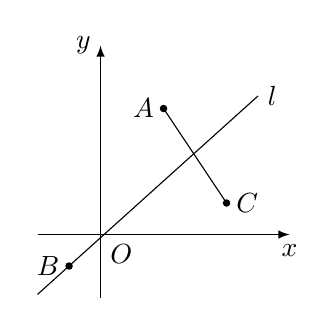
\begin{tikzpicture}[>=latex, scale = 0.4]
\draw [->] (-2,0) -- (6,0) node [below] {$x$};
\draw [->] (0,-2) -- (0,6) node [left] {$y$};
\draw (0,0) node [below right] {$O$};
\filldraw (2,4) circle (0.1) node [left] {$A$} coordinate (A);
\filldraw (-1,-1) circle (0.1) node [left] {$B$} coordinate (B);
\filldraw (4,1) circle (0.1) node [right] {$C$} coordinate (C);
\draw (A) -- (C);
\draw (B) ++ (-1,-0.9) --++ (7,6.3) node [right] {$l$};
\end{tikzpicture}
\end{center}

\begin{center}

\begin{tikzpicture}[>=latex]
\draw [very thick] (0,0) --++ (-75:2) --++ (75:2) --++ (-75:2) --++ (75:2);
\end{tikzpicture}
\end{center}


\begin{center}
\begin{tikzpicture}[>=latex,scale = 0.4]
\draw [domain = -10:10, samples= 200, very thick] plot (\x,{sqrt(210.25-pow(\x,2))-10.5});
\draw (-10,0) node [left] {$A$} -- (10,0) node [right] {$B$};
\draw (0,0) node [below] {$O$} -- (0,4) node [above] {$P$};
\draw [very thick](-6,0) node [below] {$A_1$} -- (-6,{sqrt(210.25-pow(6,2))-10.5}) node [above] {$B_1$};
\draw [very thick](-2,0) node [below] {$A_2$} -- (-2,{sqrt(210.25-pow(2,2))-10.5}) node [above] {$B_2$};
\draw [very thick](2,0) node [below] {$A_3$} -- (2,{sqrt(210.25-pow(2,2))-10.5}) node [above] {$B_3$};
\draw [very thick](6,0) node [below] {$A_4$} -- (6,{sqrt(210.25-pow(6,2))-10.5}) node [above] {$B_4$};
\end{tikzpicture}
\end{center}



\end{enumerate}

\end{document}